\chapter{Introduction}
\section{Problem Presentation}
The Vehicle Routing Problem (VRP) is an NP-optimization problem that has been of great interest for decades for both, science and industry. We got an example with Amazon that use it for the management of the deliveries from his orders around the world. The aim of our version of VRP is to find a set of minimum total cost routes for a fleet of capacitated vehicles (CVRP) based at a single depot, to serve a set of customers under the following constraints:
\begin{enumerate}
    \item each route must begin and ends at the depot node
    \item each customer/location is visited exactly once
    \item the total demand of each routes does not exceed the capacity of vehicle assigned to the route
\end{enumerate}
This type of problem is referred to a combination of two sub-problem:
\begin{enumerate}
    \item Travelling Salesman Problem (TSP) which define an Hamiltonian routes similar to the combined routes of the Vehicle Routing Problem
    \item Knapsack Problem which define constraints to manage the capacities of the vehicles in respect of the customers demands of their routes
\end{enumerate}
The VRP belongs to the category of NP-hard problems that can be exactly solved only for small instances of the problem. Therefore, many researchers have concentrated on developing heuristics algorithm to solve this problem for hard instances or find a good solution (not necessarily the optimal one). In the following section, we will explain the strategy used to solve it using a Constraint Programming approach.
\newpage
\section{Formal Problem Definition}
Let G = (V,H) be a complete directed graph with \begin{math}V \end{math} on domain \begin{math} \{1,2,3,...n, n + 1\} \end{math} as the set of nodes and H = \begin{math}\{(i,j) : i,j \in V, i \neq j\end{math}\} a set of arcs, where node n + 1 represents the depot for a fleet of v vehicles with capacities \begin{math}C_{w} > 0, w \in \{1,2..v\} \end{math}. The remaining n nodes represents the geographically position of customers. Each node of V has a location with coordinates \begin{math}(x_{i}, y_{i}) \end{math} for a node \begin{math}i \in \{1,2,3,.., n + 1\}\end{math}. Each customer \begin{math} c \in V - \{n-1\}\end{math} has a demand \begin{math} 0 < de_{c} \leq \sum_{w = 1}^{v} C_{w}.\end{math} We also have a set of distances \begin{math} D = \{d_{ij} | i,j \in V\} \end{math} represents the weight of the edge between nodes i and j.
\newline \newline Each vehicle needs to start and end his route to the depot, every customer can be visited just from a vehicle. Moreover, given \begin{math}de_{cw}\end{math} the demand \begin{math} d_{c}\end{math} satisfied by a vehicle \begin{math}w \in \{1,2...v\},\sum_{i,j \in V }d_{cw} \leq C_{w}, \forall w \in \{1,2...v\}\end{math}. \newline \newline Defined \begin{math}d_{ijw}\end{math} the distance traveled by a vehicle w and \begin{math} b_{w} \in \{0,1\}\end{math} a boolean representing if a vehicle is used or not, the aim of the problem is to minimize \begin{math}\sum_{w \in \{1,2..v\}}d_{ijw} + (\sum_{w \in \{1,2..v\}}b_{w}) * weight_{v}\end{math} with \begin{math}weight_{v}\end{math} is a constant value to balance the optimal result between the use of vehicles and the total distance traveled. [1]\newline
\newline\newline


\begin{figure}[h]
    \centering
    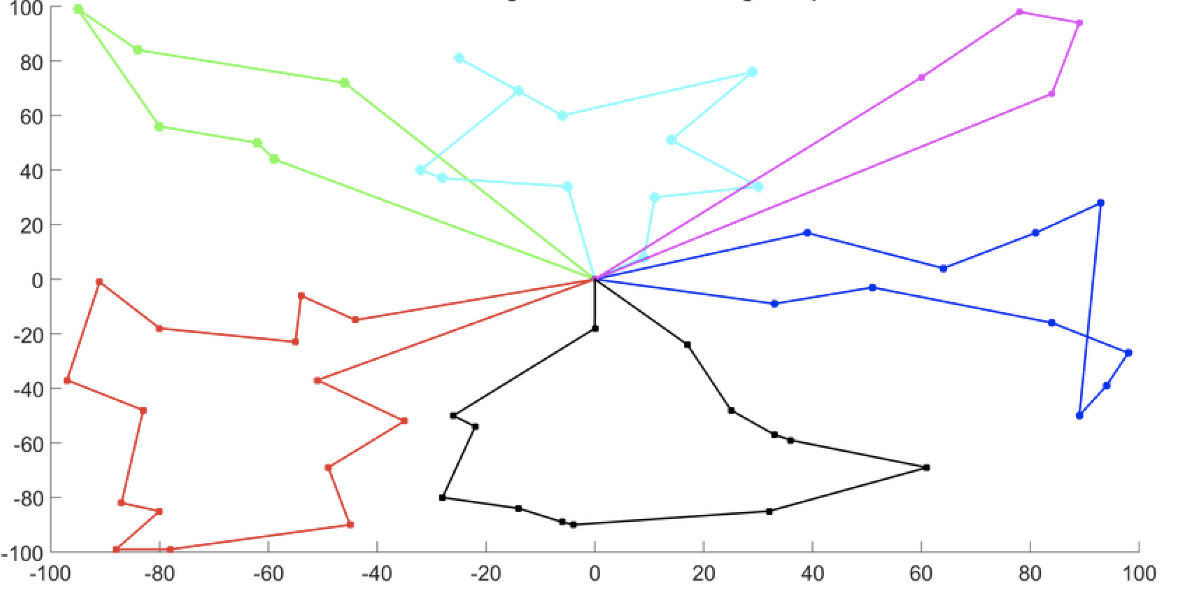
\includegraphics[width=1.0\textwidth]{images/vrp-graph.png}
    \caption{Graph of a VRP solution based on the use of 6 vehicles}
    \label{fig:mesh1}
\end{figure}
